\label{model_description}

The model used in this study was developed at Missouri University of Science and Technology.
This simulation has the express goal of being efficient while still holding true to physics models.  In order to accomplish this, it heavily leverages GPU processing by utilizing image processing techniques.  The simulation was developed with the laser \ac{DED} processes in mind, however, it was developed in a modular manner such that it can be applied to most \ac{AM} processes. 

The model is a voxel-based simulation, which forgoes the calculation of the fluid flow and focuses on heat transfer and material insertion.  This decision was based on past simulation development experience, where it was determined that the calculation of the fluid flow was the most computationally expensive part of the simulation.   

The governing equations of the model developed can be seen in Equations \ref{eqn:conduction}, \ref{eqn:conv-rad}, and \ref{eqn:laser_absorption} which describe the flow of heat from conduction, convection and radiation, and laser absorption respectively \cite{Han2012}.
	\begin{equation}
	\label{eqn:conduction}
	\centering
	\rho c_p \frac{\partial T}{\partial t}=k \left(\frac{\partial^2 T}{\partial x^2} +\frac{\partial^2 T}{\partial y^2}+\frac{\partial^2 T}{\partial z^2} \right)
	\end{equation}
		\begin{equation}
		\label{eqn:conv-rad}
		\centering
		k \frac{\partial T}{\partial n}=-h (T_s-T_a) - \varepsilon \sigma ({T_s}^4-{T_a}^4) + \phi(x, y, z) + \rho c \frac{\partial T}{\partial t}
		\end{equation}
			\begin{equation}
			\label{eqn:laser_absorption}
			\centering
			\phi(x,y,z) = H(z) \alpha \phi_0 \sqrt{1-\frac{x^2}{r_0^2} -\frac{y^2}{r_0^2}}
			\end{equation}
In these equations, $\rho$ is density, $c_p$ is specific heat, $k$ is thermal conductivity, $h$ is convection coefficient, $\varepsilon$ is emissivity, $\sigma$ is Stefan-Boltzmann constant, n is the unit (outward) normal vector of a point at location (x,y,z) that is located on the outer surface of the component, $r_0$ is the radius of the laser beam, $\alpha$ is the absorption of the material with respect to the laser radiation, $T_s$ is the surface temperature,
$T_a$ is the ambient temperature, $\phi_0$ is the laser power, and $H(z)$ is a step function which is 1 for the node with the largest z value in every (x, y) location and 0 elsewhere.


The main attributes of the model are its ability to predict the thermal history of a part, Figure \ref{fig:TEMP}, the phase map of the part at any given time, Figure \ref{fig:PHASE}, and a cooling rate for any section of the part, Figure \ref{fig:COOLRATE}.  This helps to give a predictor of the microstructure within the deposition which is the driving force behind the final mechanical properties. 
\begin{figure}[!htb]\centering
    \begin{subfigure}[c]{0.3\textwidth}
	\centering
	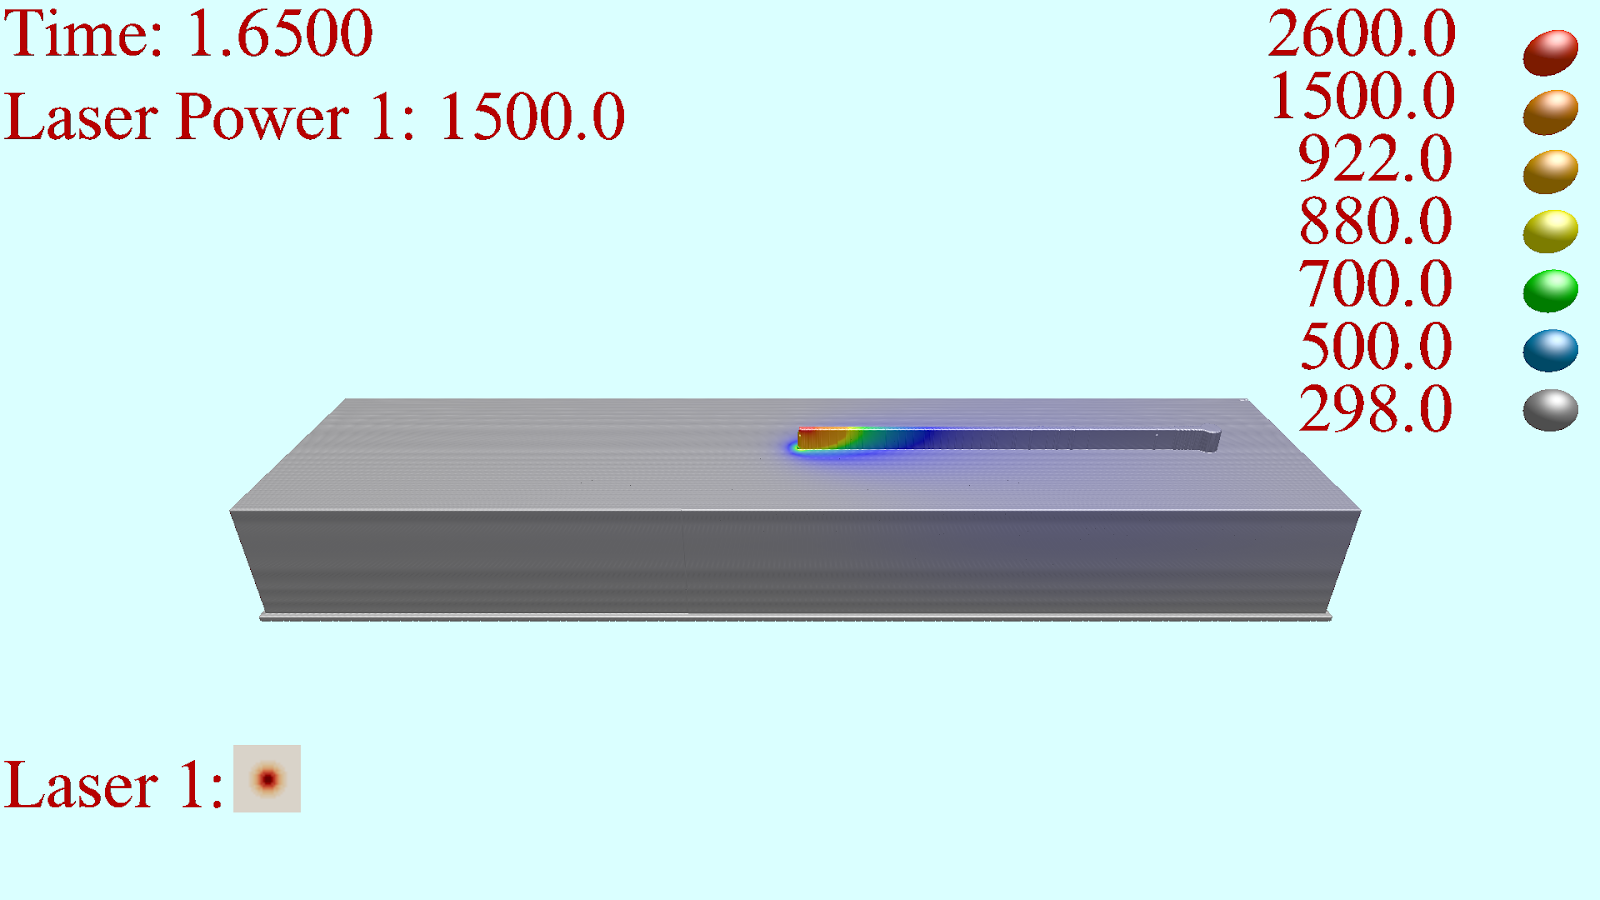
\includegraphics[width=\textwidth]{TEMP}
	\caption{Temperature profile}
	\label{fig:TEMP}
    \end{subfigure}
        \begin{subfigure}[c]{0.3\textwidth}
    	\centering
    	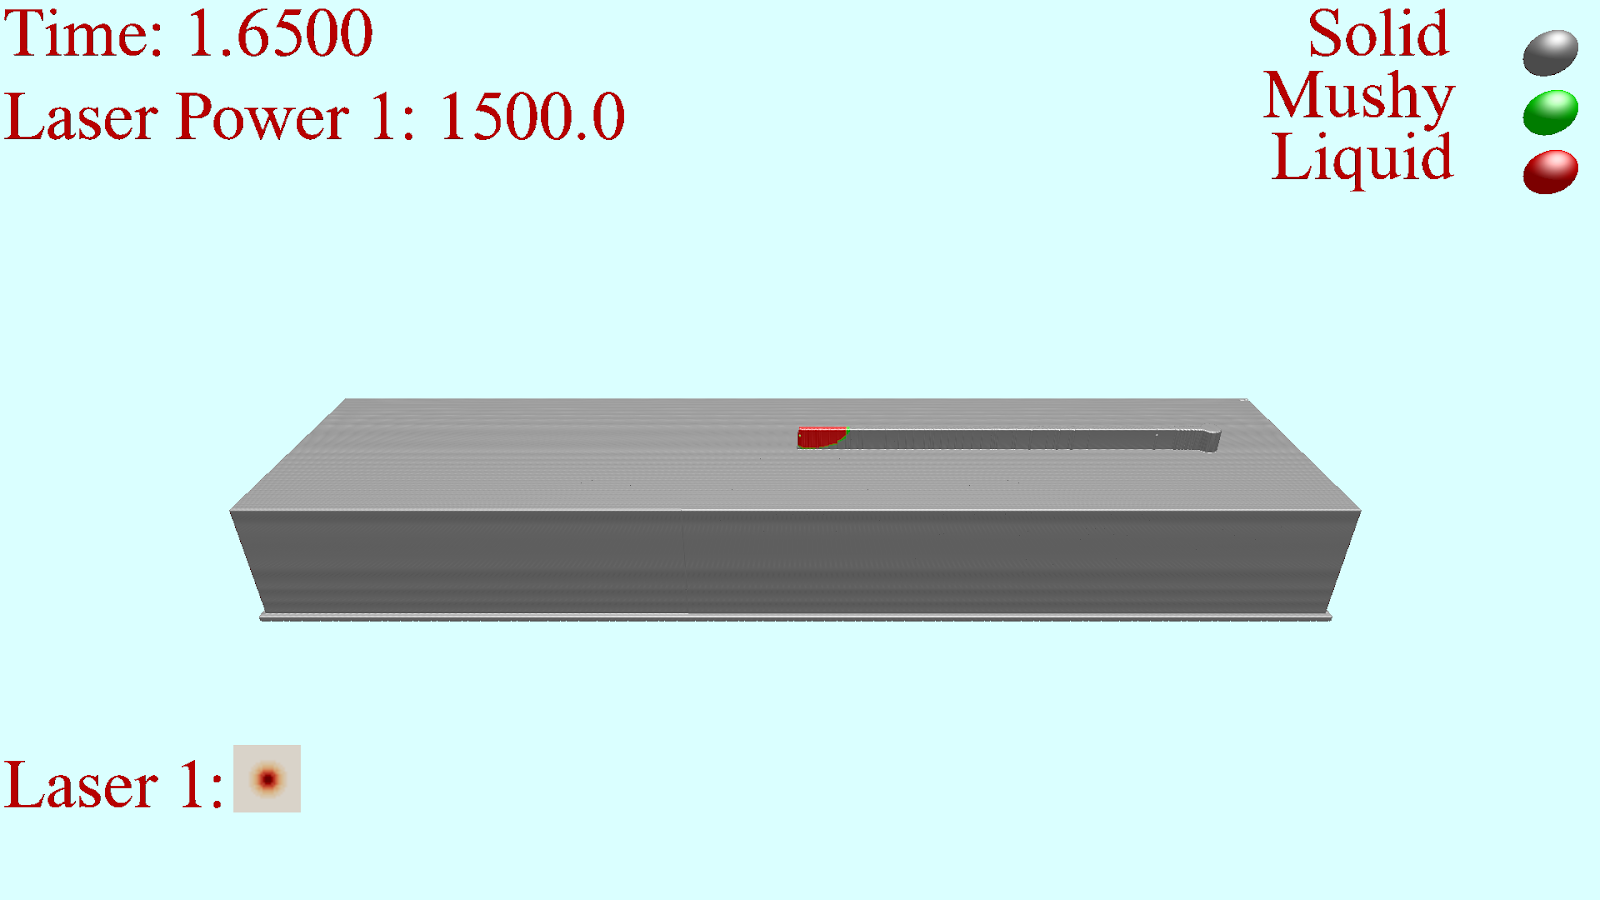
\includegraphics[width=\textwidth]{PHASE}
    	\caption{Phase map}
    	\label{fig:PHASE}
        \end{subfigure}
            \begin{subfigure}[c]{0.3\textwidth}
            \centering
        	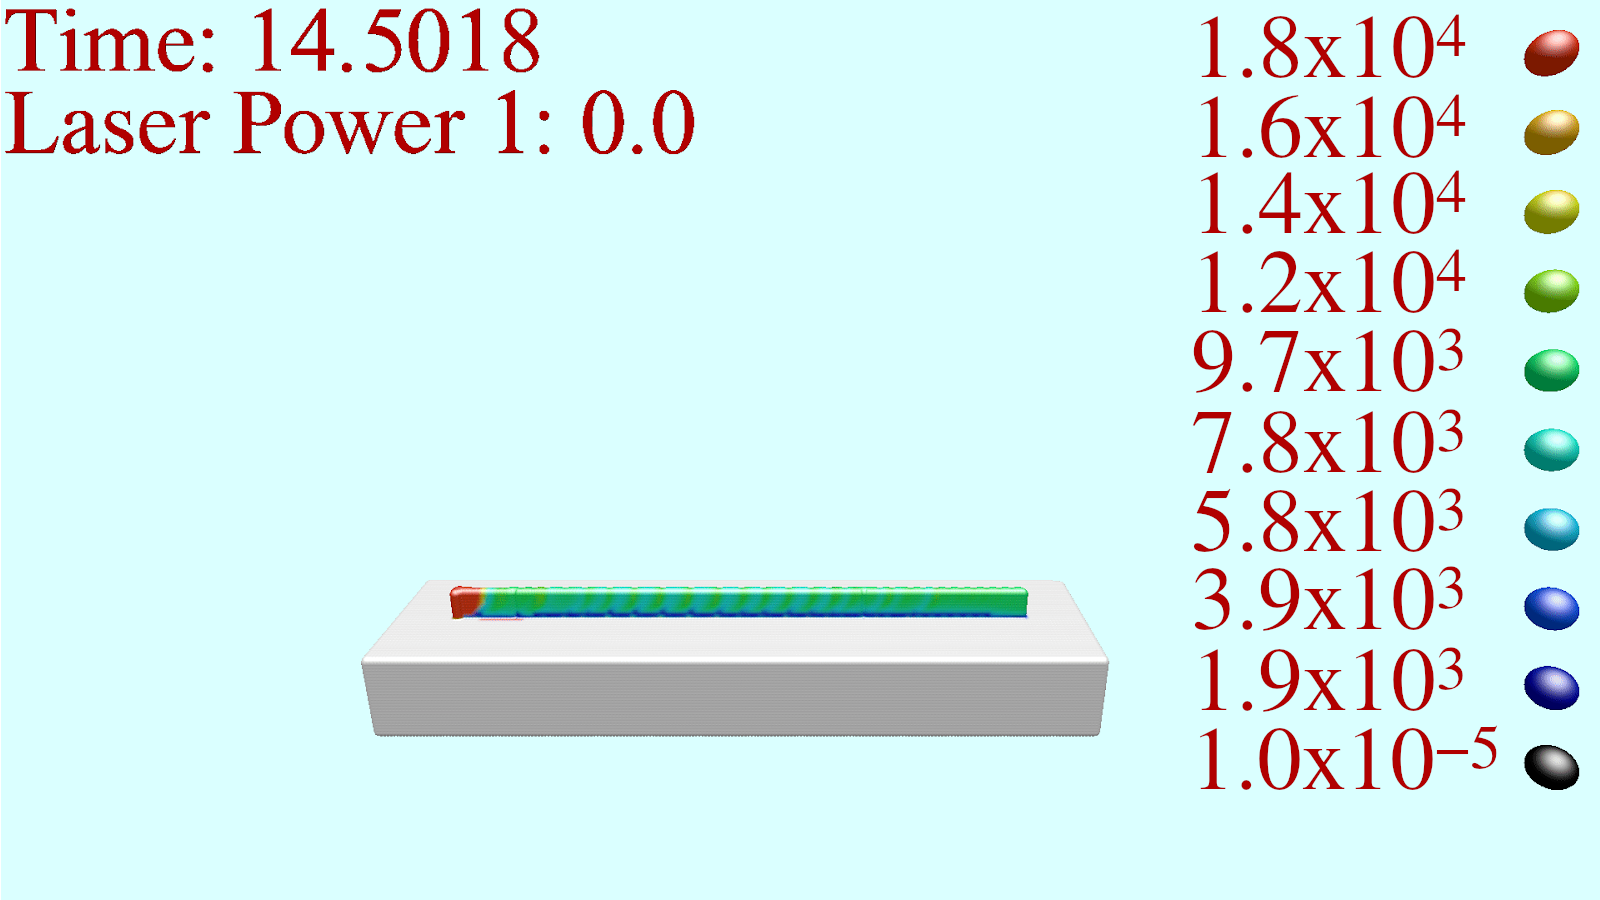
\includegraphics[width=\textwidth]{COOLRATE}
        	\caption{Cooling rate map}
        	\label{fig:COOLRATE}
            \end{subfigure}
	\caption{Examples of data maps which can be expected from the simulation.}
	\label{fig:data_maps}	
\end{figure}
Additionally, the laser in the simulation is modeled in 3-D to be able to take into account the beam quality using the \ac{BPP} reported by the manufacturer and shown in Equation \ref{eqn:bpp}, where $\theta$ and $w_0$ are the divergence angle and the beam waist respectively.
\begin{equation}\label{eqn:bpp}
	BPP = 0.5 \theta w_0
\end{equation} 
Lastly, the model includes true ray tracing enabling shadowing of the laser, the ability to define a mass which represents the machine acting as a heat sink during the build process, and the inclusion of temperature-dependent material properties.

The main objective of the model is to accurately predict the thermal history of the build.  
In order to initially validate the models, the well-characterized and published material of Ti-64 was used.  The validation was done by scanning a laser on the surface of a substrate at three energy densities with the experimental parameters found in Table \ref{tab:ti64_parameters} and the material properties used in the simulations can be seen in Table \ref{tab:ti64_properties}.
\comment{Updated table to include the property values for Ti-64\label{rev:updatedTable}}
\begin{table}[!htb] \centering
	\caption{Simulation parameters used in Ti-64 validation}
	\label{tab:ti64_parameters}
		\begin{tabular}{|c|c|} \hline 
			Parameter & Value \\ \hline
			Resolution & 60 $\mu m$ \\ \hline
			Laser diameter & 2.0 mm \\ \hline
			Laser Profile & TEM00 \\ \hline
			Laser power & 1000 W \\ \hline
			Energy density (Equation \ref{eqn:eng_density}) & 13, 18, 24 $\frac{W}{mm^3/sec}$ \\ \hline
			Scan Length & 45 mm \\ \hline
			Substrate dimensions & 55 mm x 12.7 mm x 6.35 mm \\ \hline
		\end{tabular}
\end{table}
\begin{table}[!htb] \centering
	\caption{Ti-64 material properties used in validation}
	\label{tab:ti64_properties}
	\begin{tabular}{|c|c|c|} \hline
		Material Property & Value & Reference \\ \hline
		Solidus temperature & 1603\degree C & \cite{welschgerhard_1993} \\ \hline
		Liquidus temperature & 1650\degree C & \cite{mills_2002} \\ \hline
		Solid density & 4420.0 $\frac{kg}{m^3}$ & \cite{mills_2002} \\ \hline
		Fluid density & 3920.0 $\frac{kg}{m^3}$ & \cite{mills_2002} \\ \hline
		Specific heat &  0.4 - 1.15 $\frac{J}{gK}$ & \cite{boivineau_2006} \\ \hline
		Thermal conductivity & 5.0 - 43.0 $\frac{W}{mK}$ & \cite{boivineau_2006} \\ \hline
		Absorptivity & 0.4 & \cite{fan_2012} \\ \hline
	\end{tabular}
\end{table}


There are several representations of the energy density of a laser beam in \ac{AM} but the most appropriate method of calculating the energy for the \ac{DED} process is to use a surface energy density, Equation \ref{eqn:eng_density}, where P is laser power, A is the laser spot area, and v is the scan speed \cite{kurzynowskiEffectScanningSupport2019}.
\begin{equation}
	SED_{area} = \frac{P}{A v} \label{eqn:eng_density}
\end{equation}


In order to analyze the results, the samples from the three parameter sets were sectioned \added{using a wire \ac{EDM}}, polished \added{using an automated polisher to a mirror finish}, and etched \added[comment={Detailed Ti64 etching routine \label{ref:ti64Etch}}]{using Kroll's reagent} to make the melt track visible \added{with an optical microscope} as can be seen in Figure \ref{fig:melt_track_image}, this was done at three points along the melt length.  
\begin{figure}[!htb]
	\centering
		\begin{subfigure}{0.495\textwidth}
		\includegraphics[width=\textwidth]{melt_track_image}
		\caption{Sample image of the etched slice}
		\label{fig:melt_track_image}
		\end{subfigure}
			\begin{subfigure}{0.495\textwidth}
			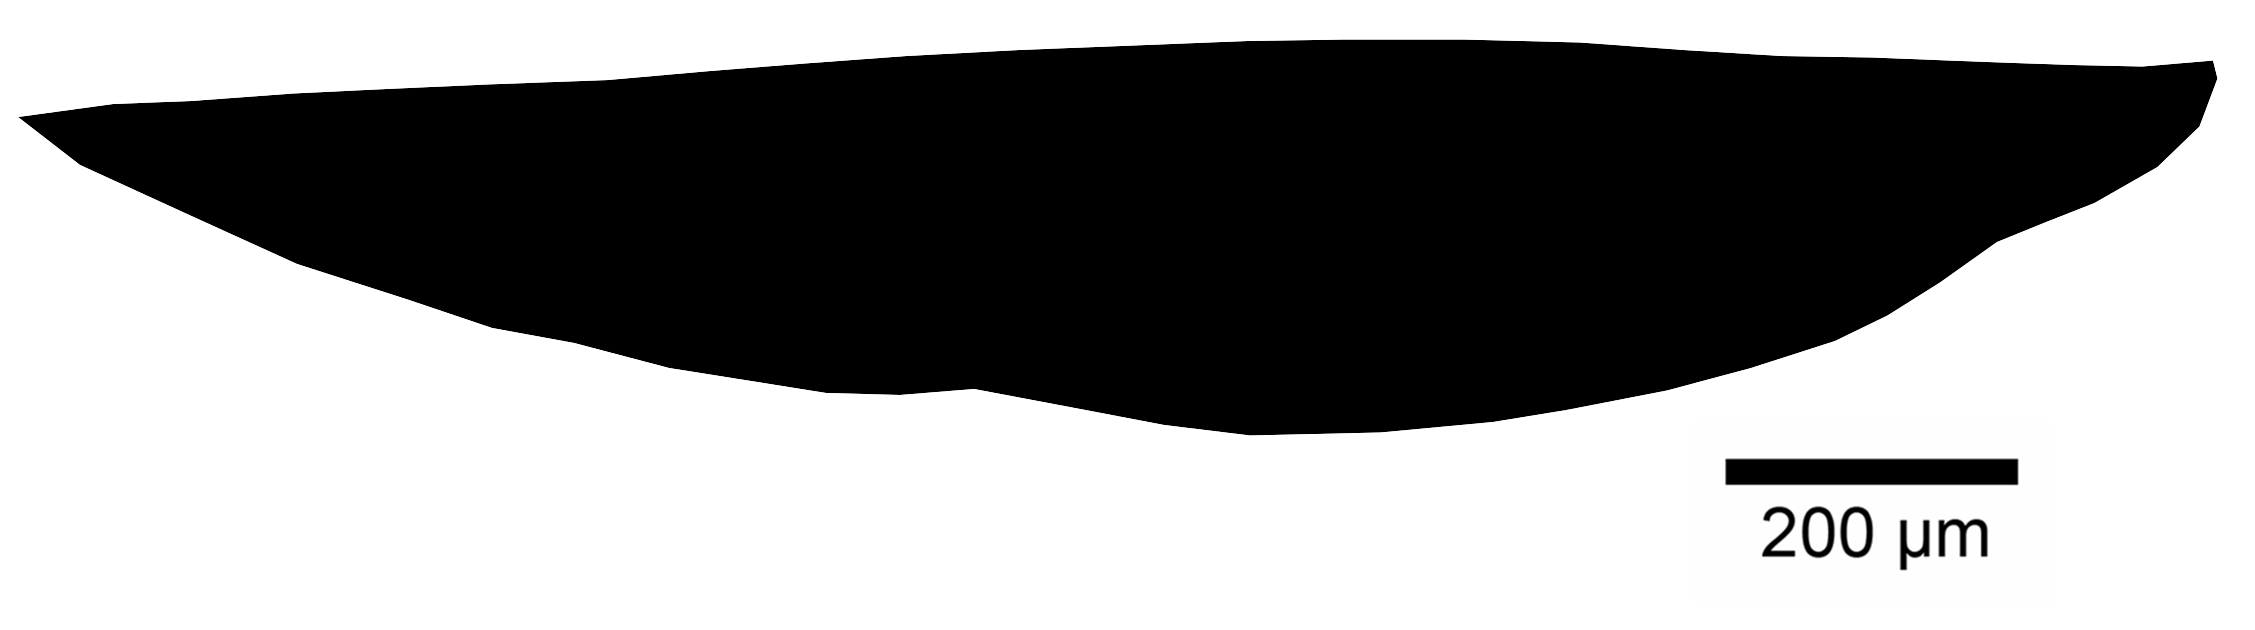
\includegraphics[width=\textwidth]{melt_track_bitmap}
			\caption{Melt pool extracted from etched slice}
			\label{fig:melt_track_bitmap}
			\end{subfigure}
	\caption{Analysis of sliced sample in Ti-64 validation}
	\label{fig:melt_track}
\end{figure}
The experiment and simulation were compared and the resulting error for the width can be seen in Figure \ref{fig:ti64_melt_track_width} and the depth can be seen in Figure \ref{fig:ti64_melt_track_depth}.
\begin{figure}[!htb]\centering
	\begin{subfigure}[c]{0.45\textwidth}\centering
	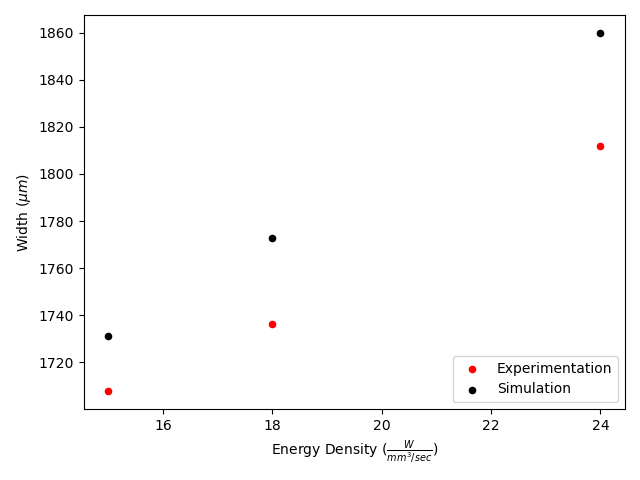
\includegraphics[width=\textwidth]{ti64_melt_track_width}
	\caption{Width}
	\label{fig:ti64_melt_track_width}
	\end{subfigure}\hfill{}
		\begin{subfigure}[c]{0.45\textwidth}\centering
		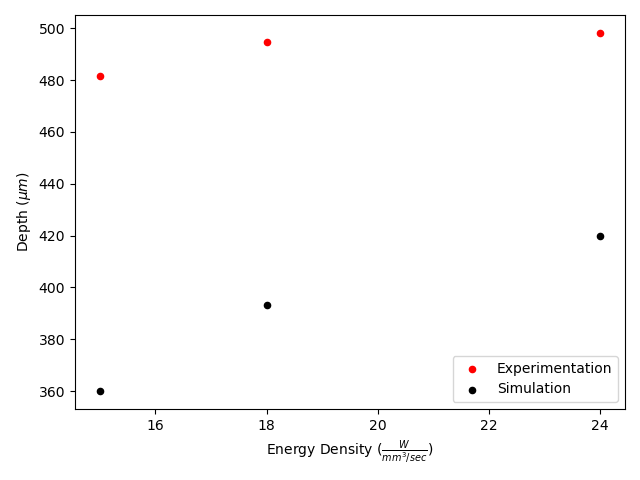
\includegraphics[width=\textwidth]{ti64_melt_track_depth}
		\caption{Depth}
		\label{fig:ti64_melt_track_depth}
		\end{subfigure}
	\caption{Comparison of simulation and experimentation in Ti-64 validation.}
	\label{fig:ti64_melt_track}
\end{figure}
The average values which are reported on the graph have an associated standard deviation of the 0.62 $\mu m$, 13.7 $\mu m$, and 7.74 $\mu m$ for the width measurements for the energy densities of 15 $\frac{W}{mm^3/sec}$, 18 $\frac{W}{mm^3/sec}$, and 24 $\frac{W}{mm^3/sec}$ respectively.  For the track depth the standard deviations are 70.2 $\mu m$, 113.7 $\mu m$, and 13.7 $\mu m$ for the energy densities of 15 $\frac{W}{mm^3/sec}$, 18 $\frac{W}{mm^3/sec}$, and 24 $\frac{W}{mm^3/sec}$ respectively.

From the plots, it can be seen that the simulation is capable of predicting the width within 3\% error and the depth error is between 15\% and 25\%.  The error in the width is very acceptable at less than 3\%.
However, the error in the depth is larger due to the resolution (voxel size) of the simulation chosen and its relative size to the depth.  This error, of approximately 20\%, for the depths which range from 450-500 $\mu m$ is 1.3-1.7 times the resolution, 60 $\mu m$, of the simulation.  Since the trends of the simulation and experimentation match and the error is within two resolution distances the 20\% error in the depth is considered acceptable as well. 
This shows that the mathematical models developed are accurate and if the material property is well characterized, the simulation will produce accurate results.

